% This file was created by matlab2tikz.
%
%The latest updates can be retrieved from
%  http://www.mathworks.com/matlabcentral/fileexchange/22022-matlab2tikz-matlab2tikz
%where you can also make suggestions and rate matlab2tikz.
%
\definecolor{mycolor1}{rgb}{0.00000,0.44700,0.74100}%
\definecolor{mycolor2}{rgb}{0.85000,0.32500,0.09800}%
\definecolor{mycolor3}{rgb}{0.92900,0.69400,0.12500}%
\definecolor{mycolor4}{rgb}{0.49400,0.18400,0.55600}%
\definecolor{mycolor5}{rgb}{0.46600,0.67400,0.18800}%
%
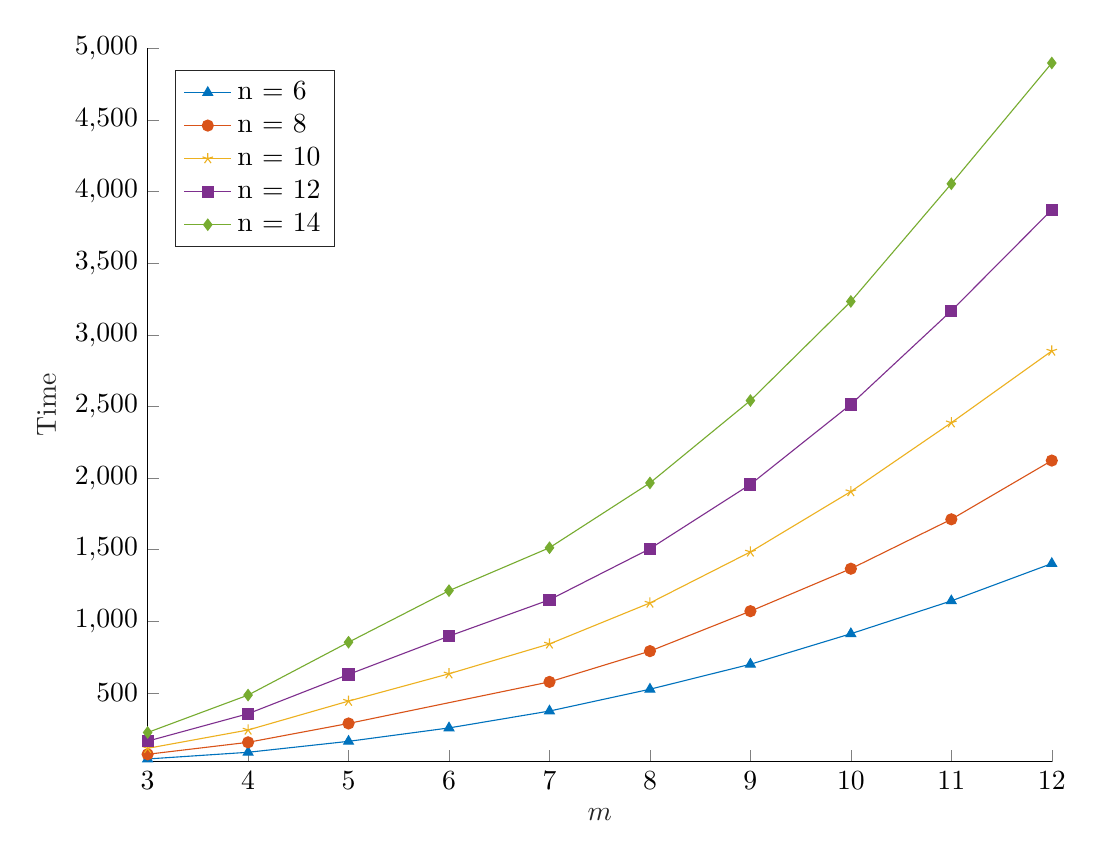
\begin{tikzpicture}

\begin{axis}[%
width=4.521in,
height=3.566in,
at={(0.758in,0.481in)},
scale only axis,
%xmode=log,
xmin=3,
xmax=12,
xminorticks=true,
xlabel style={font=\color{white!15!black}},
xlabel={$m$},
%ymode=log,
ymin=20,
ymax=5000,
yminorticks=true,
ylabel style={font=\color{white!15!black}},
ylabel={Time},
axis background/.style={fill=white},
title style={font=\bfseries},
%title={Average ticks until solution as a function of m. On n 	imes m grid. (k = 5)},
axis x line*=bottom,
axis y line*=left,
legend style={at={(0.03,0.97)}, anchor=north west, legend cell align=left, align=left, draw=white!15!black}
]
\addplot [color=mycolor1, mark=triangle*]
  table[row sep=crcr]{%
3	39.144\\
4	85.796\\
5	162.252\\
6	255.808\\
7	373.7\\
8	525.994\\
9	700.504\\
10	913.534\\
11	1142.86\\
12	1403.644\\
};
\addlegendentry{n = 6}

\addplot [color=mycolor2, mark=*]
  table[row sep=crcr]{%
3	71.86\\
4	155.35\\
5	287.108\\
7	577.234\\
8	792.134\\
9	1071.09\\
10	1367.508\\
11	1712.592\\
12	2122.772\\
};
\addlegendentry{n = 8}

\addplot [color=mycolor3, mark=star]
  table[row sep=crcr]{%
3	113.408\\
4	241.504\\
5	443.204\\
6	633.95\\
7	842.328\\
8	1128.47\\
9	1484.792\\
10	1906.444\\
11	2386.962\\
12	2887.796\\
};
\addlegendentry{n = 10}

\addplot [color=mycolor4, mark=square*]
  table[row sep=crcr]{%
3	163.68\\
4	354.946\\
5	629.508\\
6	896.894\\
7	1150.52\\
8	1507.108\\
9	1956.194\\
10	2514.728\\
11	3168.338\\
12	3873.65\\
};
\addlegendentry{n = 12}

\addplot [color=mycolor5, mark=diamond*]
  table[row sep=crcr]{%
3	223.98\\
4	485.216\\
5	854.35\\
6	1214.208\\
7	1513.966\\
8	1966.402\\
9	2541.63\\
10	3233.688\\
11	4055.356\\
12	4898.584\\
};
\addlegendentry{n = 14}

\end{axis}
\end{tikzpicture}%